\section{Background}
\label{sec:introduction:background}

This study focuses on character recognition in unstructured scenes (Figure~\ref{fig:introduction:background:sample_rbns}): specifically, short, alphanumeric number sequences. Previous works present methods to extract these sequences in various areas, namely: \gls{lpr} systems \citep{CanoPerez:2003fq,Anagnostopoulos:2006wv}; \gls{tsr} \citep{Eichner:2008dw,Kundu:2015vq,Seo:2015ez, Lian:2016dc}; and, street number recognition, specifically a study by \citet{Netzer:2011to}, using Google Street View\footnoteurl{https://www.google.com/streetview/}{13 May 2017} to determine the numerical value of street numbers. Figure~\ref{fig:sample_sequences} highlights typical usage of these sequences.

Different applications apply varying methods to parse short alphanumeric characters. There are typically two stages of any parsing method: \textit{detection} and \textit{recognition}. Detection refers to locating possible candidates and recognition refers to the representation of the text itself. Detection techniques usually are categorised as either \gls{cc}-based or learning or texture-based. CC-based detection will typically use a set of distinct properties on the image to detect relevant areas (such as width, stroke and colour) while learning-based feed images into a classifier that can distinguish candidates from false positives. The recognition phase can typically be achieved using \glsreset{ocr}\gls{ocr} engines (such as Tesseract\footnoteurl{https://github.com/tesseract-ocr/tesseract}{14 May 2017}) \citep{Benami:2012jf}, machine learning algorithms \citep{Kundu:2015vq, Netzer:2011to, Lee:1994jz} or deep-learning \glspl{nn} to classify detected regions \citep{Sermanet:2011ui, Lian:2016dc, Jin:2014jn}.

{
  \itshape
  This study proposes the development of a learning-based detection and recognition pipeline using deep-learning neural networks within the context of unstructured photos, with a focus on marathon \glspl{rbn}\footnote{While referred to as numbers, some \glspl{rbn} have alphabetic identifiers in them.}, as shown in Figure~\ref{fig:sample_rbns}.
}

\newpage
\begin{figure}[h!]
  \centering
  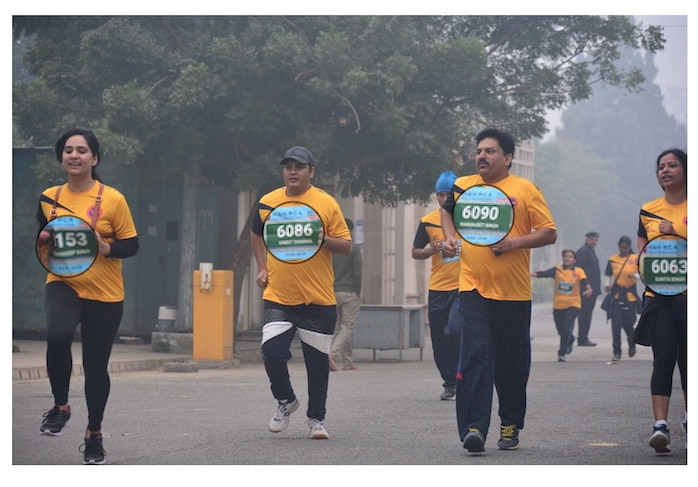
\includegraphics[width=0.7\textwidth]{images/introduction/rbn}
  \caption[Sample racing bib numbers]{Four \glspl{rbn} in a sample marathon photo.}
  \label{fig:introduction:background:sample_rbns}
\end{figure}
\vspace{\fill}
\begin{figure}[h!]
  \centering
  \begin{subfigure}[b]{0.4\textwidth}
    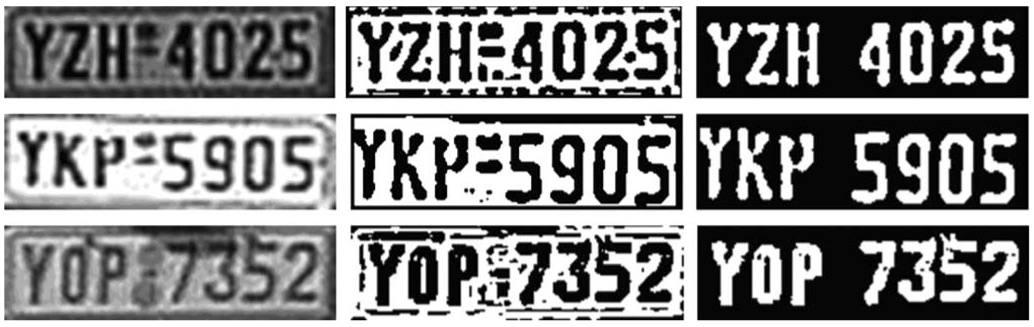
\includegraphics[width=\textwidth]{images/introduction/lpr}
    \caption{\footnotesize Successful LPR character segmentation \citep{Anagnostopoulos:2006wv}. \textit{Left to right}: original image; region segmentation; character segmentation after negation, height and orientation measurements.}
  \end{subfigure}
  \hspace{0.05\textwidth}
  \begin{subfigure}[b]{0.4\textwidth}
    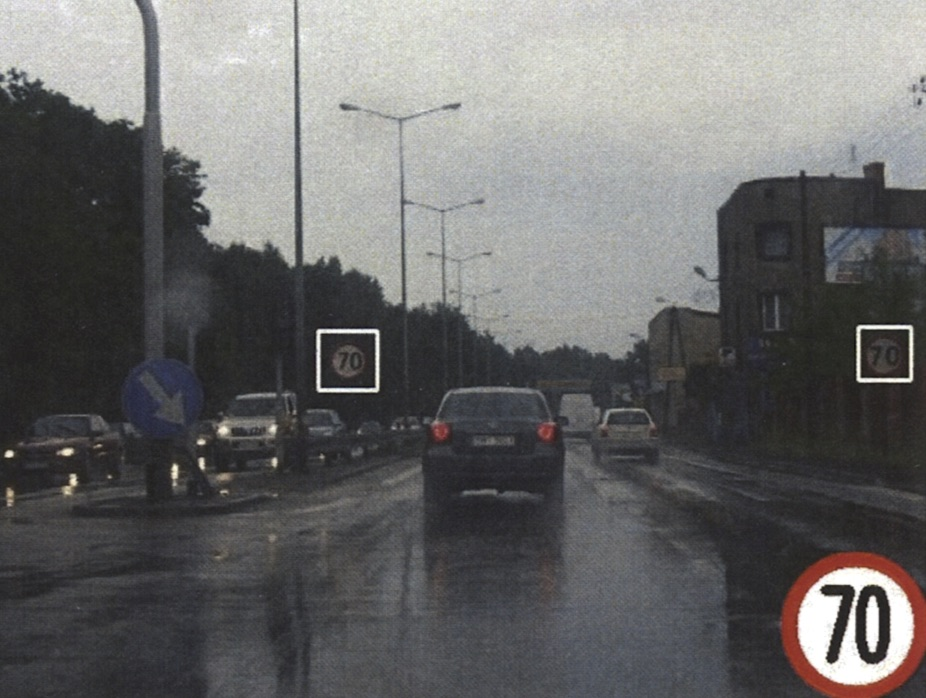
\includegraphics[width=\textwidth]{images/introduction/tsr}
    \caption{\footnotesize Successful recognition of speed sign digits shown in \citet{Eichner:2008dw}.}
  \end{subfigure}\\
  \vspace{1cm}
  \begin{subfigure}[b]{0.4\textwidth}
    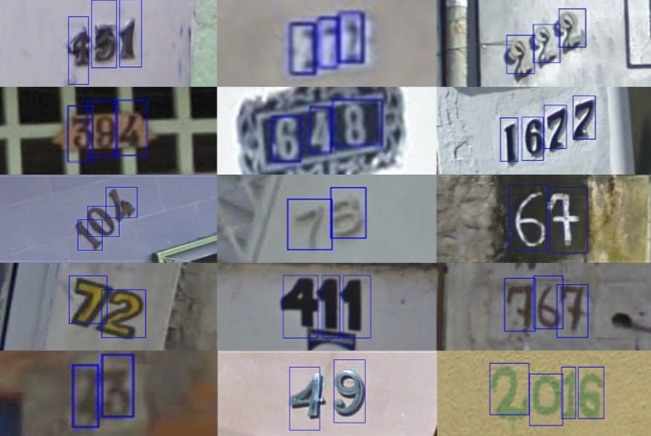
\includegraphics[width=\textwidth]{images/introduction/streetview}
    \caption{\footnotesize Localisation of digits found from varying street view house numbers using the worker described in \citet{Netzer:2011to}.}
  \end{subfigure} 
  \caption[Alphanumeric sequences observed in literature]{Various sample alphanumeric sequences observed in literature.}
  \label{fig:sample_sequences}
\end{figure}

\clearpage